\documentclass[a4paper, 11pt]{article}
\usepackage[top=3cm, bottom=3cm, left = 2cm, right = 2cm]{geometry} 
\geometry{a4paper} 
\usepackage[utf8]{inputenc}

\usepackage{graphicx} 
\usepackage{amsmath,amssymb}  
\usepackage{bm}  

%\hypersetup{linkcolor=black,citecolor=black,filecolor=black,urlcolor=black} % black links, for printed output
\usepackage{memhfixc} 

\usepackage[skip=0.333\baselineskip]{caption}
\usepackage{subcaption}
\usepackage{float}


\title{\textbf{Evaluation of CAD Algorithms}}

\author{Mohamed Ahmed Abdullah Mahmoud Mustafa}

\begin{document}


\maketitle


\section*{Introduction}

The program evaluates and tests some algorithms and finds the best evaluation measure for it with different photos.

\section*{The ROC Curves for All 4 Images}

\begin{figure}[hbt!]

\begin{subfigure}{.4\linewidth}
  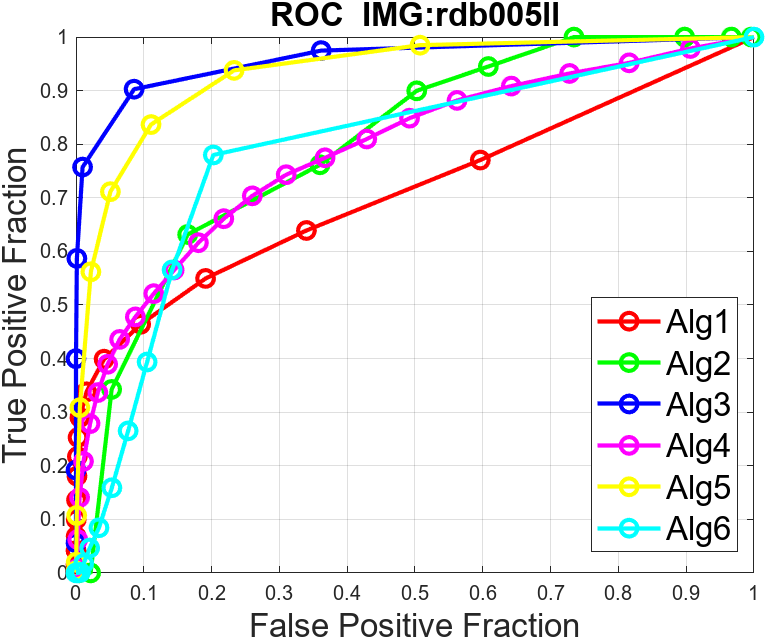
\includegraphics[width=\linewidth]{src/rdb005ll.png}
  \caption{}
  \label{MLEDdet}
\end{subfigure}\hfill % <-- "\hfill"
\begin{subfigure}{.4\linewidth}
  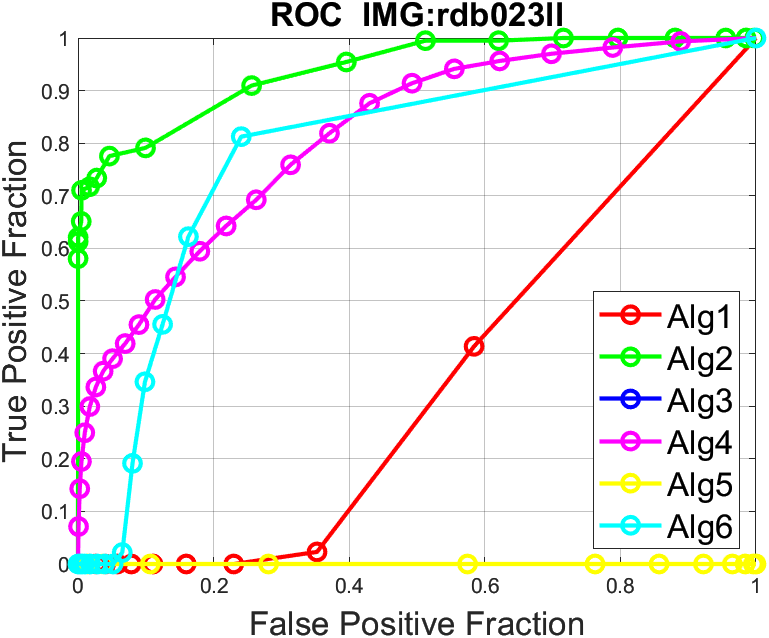
\includegraphics[width=\linewidth]{src/rdb023ll.png}
  \caption{}
  \label{energydetPSK}
\end{subfigure}

\medskip % create some *vertical* separation between the graphs
\begin{subfigure}{.4\linewidth}
  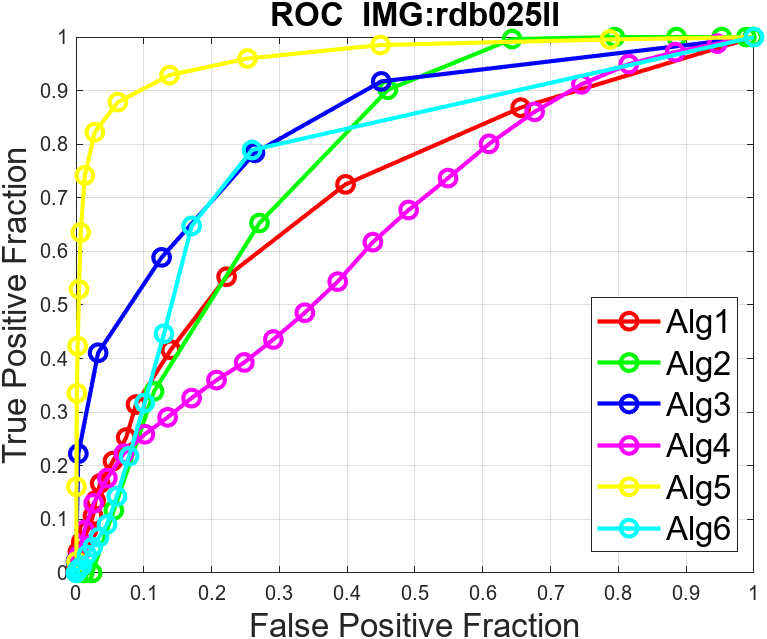
\includegraphics[width=\linewidth]{src/rdb025ll.png}
  \caption{}
  \label{velcomp}
\end{subfigure}\hfill % <-- "\hfill"
\begin{subfigure}{.4\linewidth}
  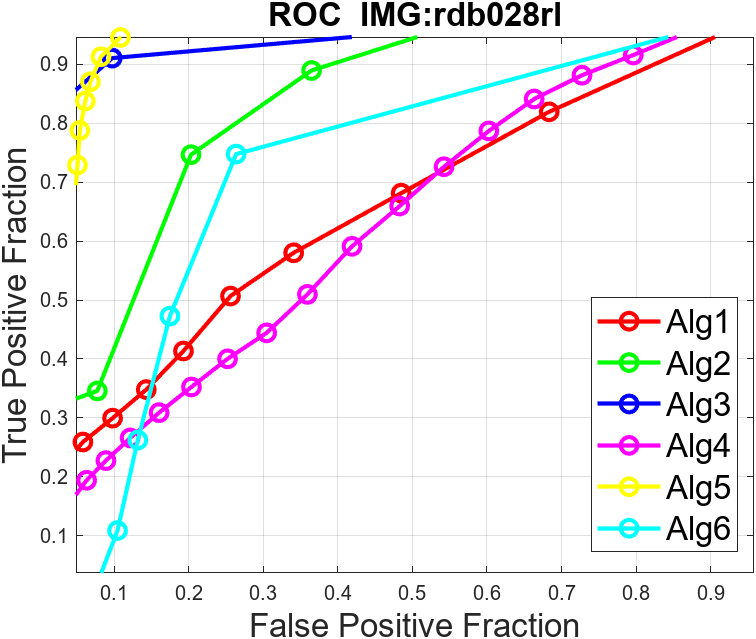
\includegraphics[width=\linewidth]{src/rdb028rl.png}
  \caption{}
  \label{estcomp}
\end{subfigure}

\caption{R.O.C. for 4 images}
\label{fig:roc}
\end{figure}


%%%%%%%%%%%%%%%%%


\section*{The Results of the 2D Evaluation \cite{wikipedia_2022} \cite{wikipedia_2023}} 

\begin{table}[h!]
\centering
\begin{tabular}{|c|c|c|c|c|c|c|}
\hline
{} & \textbf{Alg1} & \textbf{Alg2} & \textbf{Alg3} & \textbf{Alg4} & \textbf{Alg5} & \textbf{Alg6} \\
\hline
\textbf{Area Under the curve} & 0.7122 & 0.8002 & \textbf{0.9587} & 0.7888 & 0.9340 & 0.7862 \\
\hline
\textbf{Jaccard} & 0.1419 & 0.0440 & \textbf{0.7257} & 0.1230 & 0.2844 & 0.0752 \\
\hline
\textbf{Dice} & 0.2485 & 0.0843 & \textbf{0.8410} & 0.2191 & 0.4429 & 0.1400 \\
\hline
\textbf{Hausdorff Distance} & {9.2736} & {13.5647} & \textbf{4.4721} & {10.0995} & {5.7446} & {9.7980} \\
\hline
\end{tabular}
\caption{\label{tab:2d_evaluation1} 2D Evaluation for rdb005ll.png}
\end{table}

The best algorithm as \ref{tab:2d_evaluation1} shows is \text{Alg3} because its AUC is larger than AUC of other algorithms, in addition to Jaccard and Dice similarity, and the Hausdorff Distance is smaller than other algorithms.

\begin{table}[h!]
\centering
\begin{tabular}{|c|c|c|c|c|c|c|}
\hline
{} & \textbf{Alg1} & \textbf{Alg2} & \textbf{Alg3} & \textbf{Alg4} & \textbf{Alg5} & \textbf{Alg6} \\
\hline
\textbf{Area Under the curve} & {0.3459} & \textbf{0.9390} & {0.0} & {0.8143} & {0.0} & {0.7816} \\
\hline
\textbf{Jaccard} & {0.0008} & \textbf{0.1092} & {0.0} & {0.0913} & {0.0} & \textbf{0.0331} \\
\hline
\textbf{Dice} & {0.0015} & \textbf{0.1968} & {0.0} & {0.1673} & {0.0} & {0.0641} \\
\hline
\textbf{Hausdorff Distance} & {11.4018} & {9.7468} & \textbf{7.6811} & {10.3441} & \textbf{7.6811} & {12.6886} \\
\hline
\end{tabular}
\caption{\label{tab:2d_evaluation2} 2D Evaluation for rdb023ll.png}
\end{table}

The best algorithm as \ref{tab:2d_evaluation2} shows is \textbf{Alg2} because its AUC is larger than the AUC of other algorithms.

\begin{table}[h!]
\centering
\begin{tabular}{|c|c|c|c|c|c|c|}
\hline
{} & \textbf{Alg1} & \textbf{Alg2} & \textbf{Alg3} & \textbf{Alg4} & \textbf{Alg5} & \textbf{Alg6} \\
\hline
\textbf{Area Under the curve} & {0.7133} & {0.7701} & {0.8364} & {0.6439} & \textbf{0.9630} & {0.7726} \\
\hline
\textbf{Jaccard} & \textbf{0.4684} & {0.0626} & {0.3479} & {0.1013} & {0.4280} & {0.1070} \\
\hline
\textbf{Dice} & \textbf{0.6380} & {0.1179} & {0.5162} & {0.1839} & {0.5994} & {0.1933} \\
\hline
\textbf{Hausdorff Distance} & \textbf{7.9373} & {17.4642} & {11.1803} & {11.9164} & {8.3066} & {14.5945} \\
\hline
\end{tabular}
\caption{\label{tab:2d_evaluation3} 2D Evaluation for rdb025ll.png} 
\end{table}

The best algorithm as \ref{tab:2d_evaluation3} shows is \textbf{Alg5} because its AUC is larger than the AUC of other algorithms, in addition to its Jaccard and Dice distances is a 2nd smaller distance.
 

\begin{table}[h!]
\centering
\begin{tabular}{|c|c|c|c|c|c|c|}
\hline
{} & \textbf{Alg1} & \textbf{Alg2} & \textbf{Alg3} & \textbf{Alg4} & \textbf{Alg5} & \textbf{Alg6} \\
\hline
\textbf{Area Under the curve} & {0.6599} & {0.8419} & {0.9485} & {0.6356} & \textbf{0.9588} & {0.7205} \\
\hline
\textbf{Jaccard} & {0.3297} & {0.0828} & \textbf{0.7260} & {0.2491} & {0.5248} & {0.0983} \\
\hline
\textbf{Dice} & {0.4959} & {0.1529} & \textbf{0.8412} & {0.3988} & {0.6884} & {0.1791} \\
\hline
\textbf{Hausdorff Distance} & {8.0000} & {16.0624} & {6.2450} & {9.4868} & \textbf{6.0828} & {12.6095} \\
\hline
\end{tabular}
\caption{\label{tab:2d_evaluation4} 2D Evaluation for rdb028rl.png}
\end{table}

The best algorithm as \ref{tab:2d_evaluation4} shows is \textbf{Alg5} because its AUC is larger than the AUC of other algorithms, in addition to its Jaccard and Dice distances is a 2nd smaller distance.

%%%%%%%%%%%%%%%%%

\pagebreak

\section*{The Results of the 3D Evaluation}

\begin{table}[h!]
\centering
\begin{tabular}{|c|c|c|c|}
\hline
{} & \textbf{Jaccard Index Mean} & \textbf{Dice Index Mean} & \textbf{Hausdorff Distance Mean} \\
\hline
\textbf{Measures} & \textbf{0.2171} & \textbf{0.2869} & \textbf{1.4502} \\
\hline
\end{tabular}
\caption{\label{tab:2d_evaluation} 3D Evaluation}
\end{table}

%%%%%%%%%%%%%%%%%
\section*{The Best Evaluation Measure}

 It depends on the input Data-set, There is no evaluation measure that is best for all cases, but each measure has some advantages and some disadvantages, and in general, the engineer must make a trade-off according to the application that he is about to evaluate.

%%%%%%%%%%%%%%%%%
\section*{The Troubles I Have Encountered}

\begin{itemize}
    \item Dealing With Notebook in Matlab, the performance is prolonged.
    \item Can't use built-in trapezoid function in Matlab.
    \item Calculating Confusion Matrix parameters for 3D evaluation in one line.
\end{itemize}


\bibliographystyle{apalike}
% \bibliography{references}  % need to put BibTeX references in references.bib 
\bibliography{references}

\end{document}